\documentclass[12pt,oneside]{book}

%--------------------------------------------------------
% TABLE PACKAGE
%--------------------------------------------------------
\usepackage{multirow}
\usepackage{tabulary}

%--------------------------------------------------------
% Formatting Setup
%--------------------------------------------------------
\usepackage{indentfirst}
\usepackage{hyperref}
\hypersetup{hidelinks,backref=true,pagebackref=true,hyperindex=true,colorlinks=false,breaklinks=true,urlcolor= ocre,bookmarks=true,bookmarksopen=false,pdftitle={Title},pdfauthor={Isro Hidayat}}
\usepackage[top=3cm, bottom=3cm, left=4cm, right=3cm]{geometry}
\usepackage{fontspec}
\setmainfont{Times New Roman}

%-------------------------------------------------------
% SOURCE CODE Package
%-------------------------------------------------------
\usepackage{listings}
\usepackage{color}

%---------------------------------------------------------
% LIST Customizing Package
%---------------------------------------------------------
\usepackage{enumitem}
\setlist{nolistsep}
%-------------------------END LIST------------------------

%---------------------------------------------------------
% PICTURE IMPORT & CUSTOMIZE PACKAGE
%---------------------------------------------------------
\usepackage{graphicx}
\graphicspath{{Gambar/}} %Untuk menentukan direktori gambar
\usepackage{float}

%---------------------------------------------------------
% SOURCE CODE Setup & Customize LISTINGS Package
%---------------------------------------------------------
\definecolor{mygreen}{rgb}{0,0.6,0}
\definecolor{mygray}{rgb}{0.5,0.5,0.5}
\definecolor{mymauve}{rgb}{0.58,0,0.82}

\lstset{ %
  backgroundcolor=\color{white},   % choose the background color; you must add \usepackage{color} or \usepackage{xcolor}
  basicstyle=\footnotesize\ttfamily,        % the size of the fonts that are used for the code
  %basicstyle=10pt,
  breakatwhitespace=false,         % sets if automatic breaks should only happen at whitespace
  breaklines=true,                 % sets automatic line breaking
  captionpos=b,                    % sets the caption-position to bottom
%  commentstyle=\color{mygreen},    % comment style
  deletekeywords={...},            % if you want to delete keywords from the given language
  escapeinside={\%*}{*)},          % if you want to add LaTeX within your code
  extendedchars=true,              % lets you use non-ASCII characters; for 8-bits encodings only, does not work with UTF-8
  frame=shadowbox,	               % adds a frame around the code
  rulesepcolor=\color{mygreen},
  keepspaces=true,                 % keeps spaces in text, useful for keeping indentation of code (possibly needs columns=flexible)
%  keywordstyle=\color{blue},       % keyword style
  language=TeX,                 % the language of the code
  otherkeywords={*,...},            % if you want to add more keywords to the set
  numbers=left,                    % where to put the line-numbers; possible values are (none, left, right)
  numbersep=5pt,                   % how far the line-numbers are from the code
  numberstyle=\tiny\color{mygray}, % the style that is used for the line-numbers
  rulecolor=\color{black},         % if not set, the frame-color may be changed on line-breaks within not-black text (e.g. comments (green here))
  showspaces=false,                % show spaces everywhere adding particular underscores; it overrides 'showstringspaces'
  showstringspaces=false,          % underline spaces within strings only
  showtabs=false,                  % show tabs within strings adding particular underscores
  stepnumber=1,                    % the step between two line-numbers. If it's 1, each line will be numbered
%  stringstyle=\color{mymauve},     % string literal style
  tabsize=2,	                   % sets default tabsize to 2 spaces
  title=\lstname                   % show the filename of files included with \lstinputlisting; also try caption instead of title
}

%--------------------- End Source Code ------------------------------------------------------


%----------------------------------------------------------------------------
% Pengaturan Judul, Author, dan Cover Book
%----------------------------------------------------------------------------
\title{Belajar \LaTeXe\ Dari Awal}
\author{Isro\rq\ Hidayatulloh}
\date{06 Juli 2015}


%----------------------------------------------------------------------------
%								DOKUMEN INTI
%----------------------------------------------------------------------------
\begin{document}
\renewcommand{\contentsname}{Daftar Isi}
\renewcommand{\partname}{Bagian}
\renewcommand{\chaptername}{BAB}
\renewcommand{\figurename}{Gambar}
\renewcommand{\tablename}{Tabel}
\renewcommand{\bibname}{Daftar Pustaka}
\renewcommand{\listtablename}{Daftar Tabel}
\renewcommand{\listfigurename}{Daftar Gambar}
\setcounter{secnumdepth}{2}
\maketitle
%\newpage
\tableofcontents

\part{Tahap Pengenalan}%\index{Tahap Pengenalan}

\chapter{Apa itu \LaTeX?}
\TeX\ adalah bahasa pemrograman yang dibuat oleh Donald Knuth\footnote{\url{http://en.wikipedia.org/wiki/Donald\%20Kuth}}\ fungsinya untuk membuat dokumen yang yang baik dengan mudah. Lalu apa hubungannya dengan \LaTeX , \LaTeX\ adalah pengembangan dari \TeX\ dengan penambahan package atau style. Sehingga memberikan kemudahan untuk pembuatan dokumen yang kompleks, seperti untuk mengubah font, penambahan gambar, dan masih banyak lagi.

\section{Instalasi}
Instalasi \LaTeX\ menggunakan sistem distribusi, distribusi \LaTeX\ ini terdiri dari sekumpulan paket dan program. Berikut adalah distribusi \LaTeX\ untuk kebanyakan sistem operasi:
\begin{itemize}
	\item TeX Live\footnote{\url{http://www.tug.org/texlive/}}\ adalah kebanyakan distribusi \TeX\ untuk BSD, GNU/Linux, Mac OS X, dan Windows.
	\item MiKTeX\footnote{\url{http://www.miktex.org/}}\ adalah distribusi khusus Windows.
	\item MacTeX\footnote{\url{http://www.tug.org/mactex/}}\ distribusi khusus Mac OS turunan dari TeX Live.
\end{itemize}
Paket distribusi ini tidak mengikutsertakan editor. Kita bisa menggunakan text editor biasa untuk membuat kode sumber \LaTeX .
\subsection{Instalasi di Linux}
Linux terdiri dari banyak distro/distribusi, ada Ubuntu, Debian, Fedora, dsb. Kebanyakan distro telah mengikutsertakan distribusi TeX Live pada repositorinya. Pada Ubuntu kita bisa menggunakan aplikasi Synaptic Package Manager.
\begin{figure}[h!]
\centering
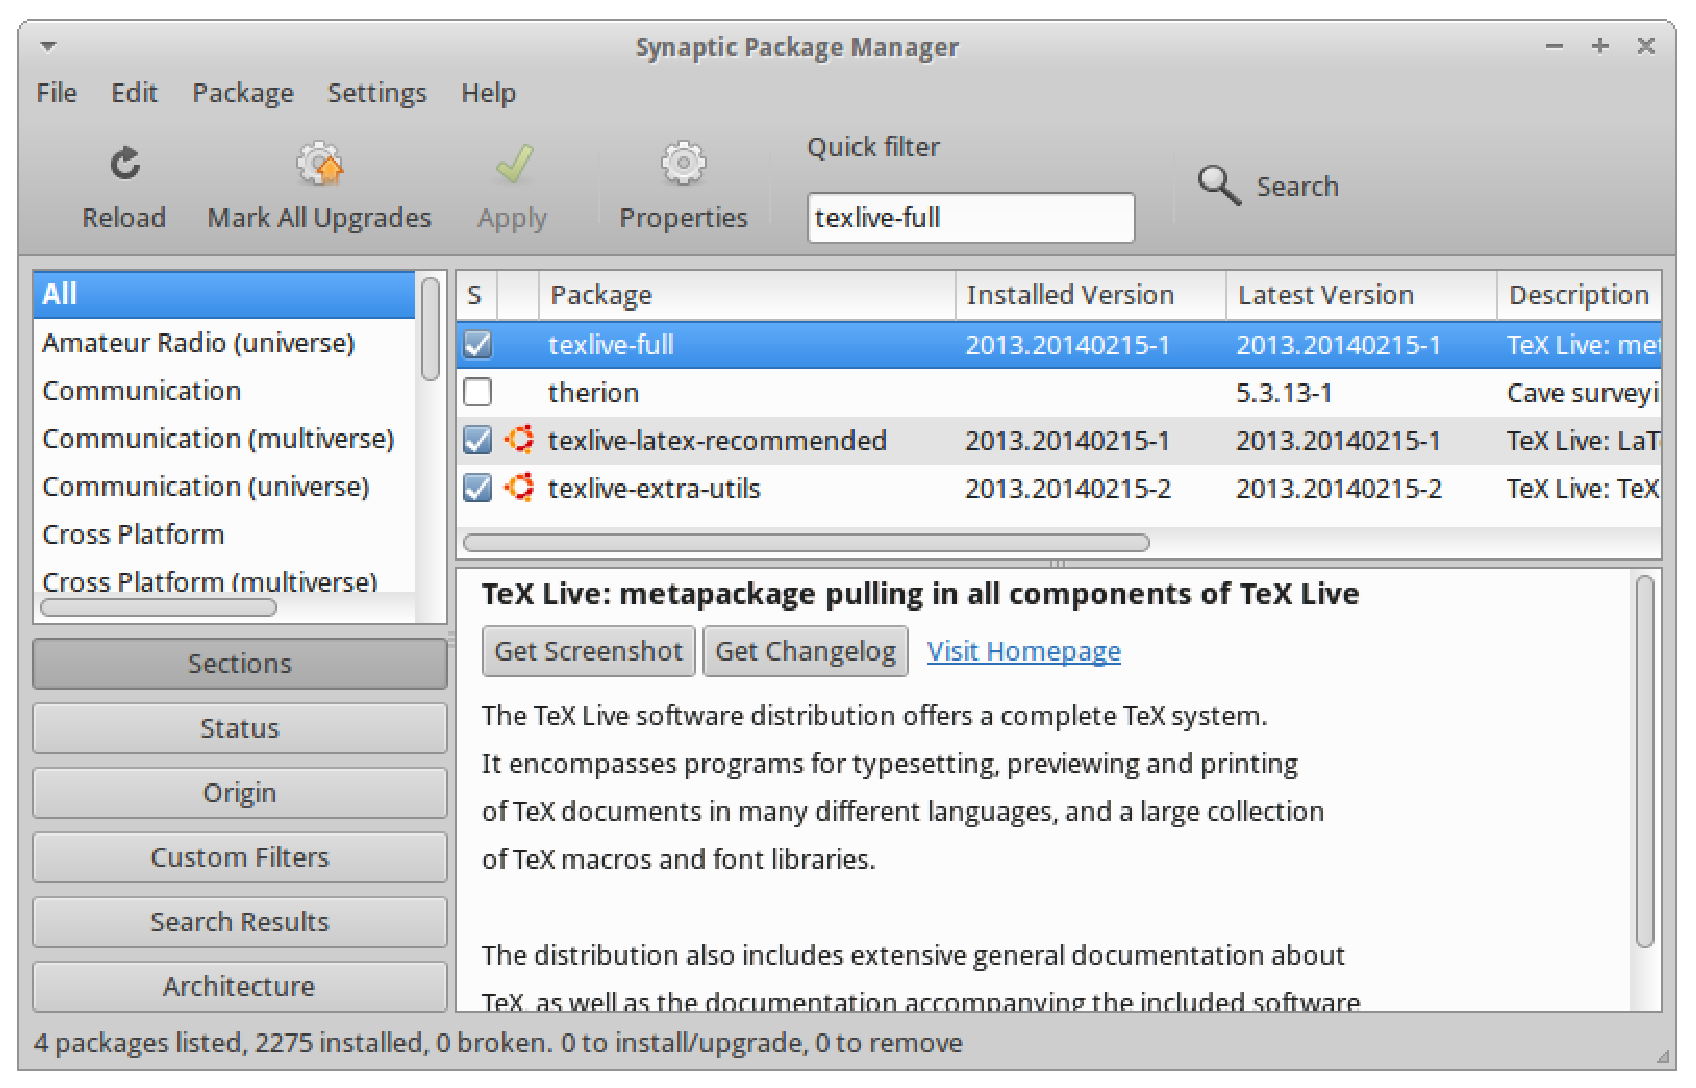
\includegraphics[scale=0.4]{Install_TexLive}
\caption{Install Texlive-full Menggunakan Synaptic}
\label{fig:install_texlive}
\end{figure}


\chapter{Dasar}
Pada bab ini kita akan mulai belajar dasar-dasar LaTeX, jadi anda harus sudah menginstall aplikasi LaTeX pada komputer. Kami menyarankan menggunakan Texmaker sebagai editor LaTeX. Karena kelengkapan dan juga kemudahan pengguanaannya. Sedangkan pada sistem operasi Windows teman-teman bisa menggunakan Texwork.
\section{Sintak \LaTeX}
\LaTeX\ mengkonversi teks sumber dikombinasikan dengan markup kedalam dokumen dengan kualitas tinggi. File input untuk \LaTeX\ adalah plain text\footnote{http://en.wikipedia.org/wiki/plain\%20text}. Bentuk umum paling sederhana adalah sebagai berikut:

\begin{lstlisting}
\documentclass{article}

\begin{document}
Hello world!
\end{document}
\end{lstlisting}

\subsection{Spasi}
Kompiler LaTeX menormalisasi spasi, baik itu berupa spasi atau tab. Meski kita membuat spasi sebanyak apapun LaTeX akan menganggapnya sebagai spasi tunggal. Begitu juga dengan ganti baris tunggal juga dianggap sebagai spasi, jika ganti baris ini dilakukan dua kali atau membuat baris kosong antar dua baris. Hal ini baru menjadikan Paragraf baru pada output.

Berikut contoh yang akan membantu anda memahamai bagaimana kerja spasi di LaTeX:

\lstinputlisting[language=TeX, caption=spasi.tex]{Contoh/spasi.tex}

Sehingga output yang didapat dari kode sumber diatas adalah:

\begin{figure}[h]
\centering
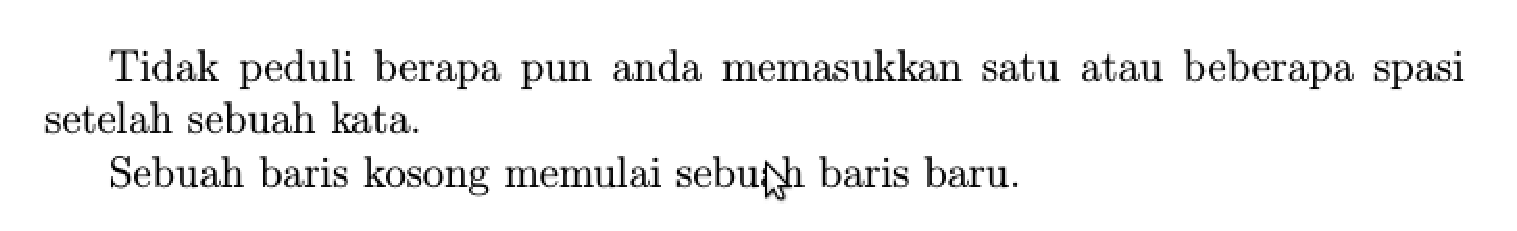
\includegraphics[scale=0.5]{spasi}
\caption{Spasi Pada LaTeX}
\label{fig:spasi}
\end{figure}

Untuk selanjutnya silahkan anda beruji coba sendiri yah.. :-). Selanjutnya adalah

\subsection{Karakter Khusus}
Karakter-karakter ini adalah karakter/huruf yang memiliki suatu arti bagi kompiler LaTeX. Jika kita tuliskan karakter-karakter ini secara langsung pada kode, maka akan menghasilkan hal yang tidak sesuai keinginan. Karakter-karakter ini adalah :
\begin{figure}[h]

\includegraphics[scale=0.5]{karakterkhusus}
\end{figure}

\lstinputlisting[language=TeX, caption=karakterkhusus.tex, firstline=4, lastline=4]{Contoh/karakterkhusus}

Karakter backslash(\textbackslash{}) tidak bisa ditambahkan dengan cara menambahkan backslash lagi setelahnya (\textbackslash{}\textbackslash{}). Cara ini digunakan untuk mengakhiri baris. Sedangkan pada karakter \textbackslash{}\^{} dan \textbackslash{}\~{} harus ditambahkan kurung kurawal, karena kalau tidak perintah ini \textbackslash{}\~{}n akan menghasilkan \~n.

\subsection{Group}
Sebuah \emph{group} pada dasarnya didefinisikan dengan sepasang kurung kurawal \{\}. Dan perintah-perintah yang ada didalamnya hanya berkerja pada group tersebut. Perintah \textbackslash{}begingroup dan \textbackslash{}endgroup merupakan perintah alternatif dari kurung kurawal. Contoh:
\begin{lstlisting}
{
\bf Yang ini BOLD
}
di sini tidak lagi
\end{lstlisting}
\begin{figure}[h]
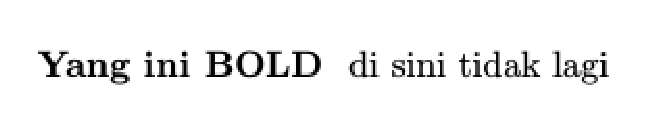
\includegraphics[scale=0.5]{group}
\end{figure}
group berguna ketika kita menginginkan suatu perintah hanya berpengaruh pada beberapa baris atau kata saja.

\subsection{Environment}
\emph{Enviroment} di LaTeX punya aturan yang mirip dengan perintah/command, biasanya environment punya pengaruh lebih luas.  Sintaks umumnya: 
\begin{lstlisting}
\begin{namaenvironment}
di sini teks yang terpengaruh oleh environment
\end{namaenvironment}
\end{lstlisting}
Diantara \texttt{\textbackslash{}begin} dan \texttt{\textbackslash{}end}\ kita dapat menambahkan perintah lain dan juga bisa nested environment(environment bertumpuk).

\subsection{Commands}
(\emph{Commands}) bersifat case sensitive dan mengikuti dua aturan berikut:
\begin{itemize}
\item diawali dengan backslash \textbackslash{} dan selanjutnya nama command yang hanya berisi hanya huruf. Command diterminasi dengan sebuah spasi, sebuah angka atau apapun selain huruf.
\item Berisi sebuah backslash \textbackslash{} dan tentunya sebuah non-huruf.
\end{itemize}
Beberapa commands butuh argumen yang diletakkan di dalam kurung kurawal \{\} setelah nama command. Juga terkadang butuh opsi tambahan yang diletakkan di dalam kurung siku [ ]. Sintaks sebagai berikut:
\begin{lstlisting}
\namacommand[opsi1,opsi2,...]{argumen1}argumen2}...
\end{lstlisting}
Kebanyakan perintah standar LaTeX punya \emph{switch}. Switch ini adalah sebuah kesamaan dari command/perintah hanya saja tidak punya argumen dan berada di dalam kurung kurawal. Jangan memanggilnya diluar kurung karena akan berpengaruh ke seluruh dokumen.\\
Contoh:\\
\begin{lstlisting}
% \emph adalah command/baris perintah, \em adalah switch
\emph{text tercetak miring}, bagian ini normal % Format Benar
{\em text tercetak miring}, bagian ini normal % Format benar

\em text tercetak miring, bagian normal % Format salah
\emph{text tercetak miring}, bagian normal % Format salah
\end{lstlisting}

\subsection{Komentar}
Jika pada input file terdapat karakter \% maka baris setelahnya tidak ikut dieksekusi, dan tidak berpengaruh pada hasil output. Biasanya digunakan untuk membuat catatan tentang perintah atau keterangan dari dokumen yang dibuat.
\lstinputlisting[language=TeX, caption=komentar.tex, firstline=4, lastline=8]{Contoh/komentar}
\begin{figure}[h]
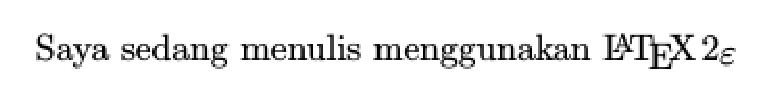
\includegraphics[scale=0.6]{komentar}
\end{figure}

Sebagai catatan bahwa karakter \% bisa digunakan untuk memisahkan kata yang panjang tanpa ada spasi atau ganti baris.

\section{Membuat Dokumen Pertama}
Sekarang saatnya membuat dokumen sederhana untuk langkah awal. Kita bisa membuat kode sumber LaTeX ini menggunakan text editor seperti Notepad++, vim, dan gedit. Namun kami sarankan untuk menggunakan editor LaTeX khusus seperti Texwork untuk Windows sedangkan untuk Linux menggunakan Texmaker.
\lstinputlisting[language=TeX, caption=assalam.tex]{Contoh/assalam}

\subsection{Apa Arti dari Kode Sumber?}
Mari kita pelajari tiap baris dari kode sumber di atas:
\begin{itemize}
\item \textbf{\texttt{\% assalam.text - Contoh pertama LaTeX}}\\
Baris pertama adalah baris komentar, baris ini tidak akan nampak dan tidak menjalankan perintah apapun. Bisa digunakan untuk memberi keterangan mengenai isi kode sumber, dan informasi tentang pengarang, dsb.
\item \textbf{ \texttt{\textbackslash{}documentclass\{article\}}}\\
Ini adalah baris perintah atau command yang memberitahukan LaTeX untuk menggunakan format dokumen \texttt{article}.
\item \textbf{\texttt{\textbackslash{}begin\{document\}}}\\
Ini adalah gerbang untuk lingkungan dokumen, Isi dokumen diletakkan setelah perintah ini. Sedangkan perintah-perintah yang berada di atasnya dinamakan \emph{preamble}.
\item \textbf{\texttt{Assalamualaikum Warahmatulloh... \% Salam Rek..! Biar beda :-)}}\\
Nah ini adalah baris yang akan nampak pada hasil akhir.
\item \texttt{\textbf{\textbackslash{}end\{document\}}}\\
Ini adalah baris penutup dari perintah \textbackslash{}begin\{document\}. Apa pun setelah perintah ini tidak akan dipedulikan.
\end{itemize}

\section{File}
\subsection{Membuat Nama File yang Baik}
Tidak semua nama file bisa digunakan, ada tata caranya. Jangan menggunakan nama file atau folder mmenggunakan spasi, kita bisa membuat nama yang panjang tapi hindari spasi. Gunakan huruf (a-z) angka (1-9) dan tanda minus (-) dan sebuah titik untuk pemisah ekstensi file. Jangan mencampur antara huruf besar dan kecil dalam satu nama, karena beberapa sistem operasi tidak memperdulikan namun yang lainnya membedakannya.

\subsection{File Tambahan}
Selain file \texttt{.tex} ada beberapa file pendukung lain, file-file ini ada yang bersifat semetara. Berikut ekstensi umum file-file di LaTeX:
\begin{center}
\begin{tabular}{|l|p{0.8\textwidth}|}
%\hline
%\textbf{Ekstensi-ekstensi File LaTeX}
\hline
\textbf{Ekstensi} & \textbf{Penjelasan}\\
\hline
.aux & File ini digunakan untuk menyimpan informasi yang berhubungan dengan cross-referense\\
\hline
.bbl & File bibliography, merupakan output dari BiBTeX dan digunakan oleh LaTeX\\
\hline
.bib & File database bibliography\\
\hline
.blg & File log dari BiBTeX\\
\hline
.bst & File Tipe/model BiBTeX \\
\hline
.cls & File class yang mendefinisikan seperti apa dokumen anda. Dipilih dengan menggunakan perintah \texttt{\textbackslash{}documentclass}.\\
\hline
.dtx & TeX terdokumentasi. Merupakan format distribusi utama dari file style LaTeX.\\
\hline
.ins & File installer untuk file \texttt{.dtx}.\\
\hline
.fd & File yang mendeskripsikan font baru agar dikenali oleh LaTeX.\\
\hline
.dvi & File Device Independent. Ini adalah output utama yang dihasilkan dari kompilasi kode sumber LaTeX menggunakan kompiler \emph{latex}. Bisa dilihat menggunakan aplikasi DVI previewer atau aplikasi-aplikasi yang medukungnya.\\
\hline
.pdf & Portable Document Format. Merupakan hasil utama dari kompilasi kode sumber LaTeX menggunakan kompiler \emph{pdflatex}. Banyak sekali aplikasi untuk menampilkan dokumen dengan ekstensi PDF, salah satunya Adobe Reader, dan Okular.\\
\hline
.log & Memberikan detil laporan selama kompiler berjalan.\\
\hline
.toc & Menyimpan semua header section. Digunakan untuk membuat daftar isi.\\
\hline
.lof & Mirip dengan.toc hanya saja untuk membuat daftar gambar (\emph{list of figures}).\\
\hline
.lot & Sama juga tapi untuk membuat daftar tabel (\emph{list of tables}).\\
\hline
.idx & Jika di dalam dokumen terdapat indeks. LaTeX menyimpan kata-kata indeks tersebut di dalam file ini. Diproses dengan menggunakan perintah makeindex.\\
\hline
.ind & File .idx yang telah diproses dan siap untuk dimasukkan ke dalam dokumen pada perputaran kompilasi selanjutnya.\\
\hline
.ilg & File log yang memberitahukan apa yang telah dilakukan oleh makeindex.\\
\hline
.sty & File makro package LaTeX. File ini bisa di-load ke dalam dokumen LaTeX menggunakan perintah \texttt{\textbackslash{}usepackage}.\\
\hline
.tex & File Input LaTeX atau TeX.\\
\hline
.out & File paket hyperref, hanya satu digunakan untuk file master.\\
\hline
\end{tabular}
\end{center}

\part{Elemen-elemen Umum}
\chapter{Struktur Dokumen}
Tujuan dari menulis adalah untuk menyampaikan apa yang kita pikirkan, informasi atau pengetahuan kepada pembaca. Pembaca akan mudah memahami jika ide/tulisan kita tertata dengan baik, dalam hal ini hasil tulisan kita terstruktur secara rapi. 

LaTeX berbeda dengan sistem penulisan yang lainnya. LaTeX menyediakan kemudahan untuk pengguna  menata dokumen mereka dengan berbagai hirarki, termasuk bab, subbab, dan paragraf.

\section{Struktur Global}
Ketika LaTeX memproses kode sumber, dia meminta kode tersebut mengikuti aturan tertentu. Oleh karena itu lah kode sumber ini harus berisi perintah
\begin{lstlisting}
\documentclass{...}

\begin{document}
...
\end{document}
\end{lstlisting}

Wilayah antara \texttt{\textbackslash{}documentclass\{...\}} dan \texttt{\textbackslash{}begin\{document\}} dinamakan \emph{preamble}. Biasanya berisi perintah yang mempengaruhi keseluruhan dokumen.

Setelah preamble adalah teks dokumen, berada diantara perintah yang menandakan dimulai dan berakhirnya suatu teks dokumen.
\begin{lstlisting}
\begin{document}
...			% Disini teks yang akan ditampilkan pada output.
\end{document}
\end{lstlisting}

\section{Preamble}
\subsection{Document class}
Ketika memproses file sumber, LaTeX perlu tahu tipe dokumen yang ingin dibuat penulis. Caranya dengan menggunakan perintah \texttt{\textbackslash{}documentclass}. Seharusnya diletakkan diawal kode input.
\begin{lstlisting}
\documentclass[option]{class}
\end{lstlisting}

\texttt{class} menentukan tipe dokumen yang akan dibuat. Misal LaTeX juga mendukung class dokumen surat(letter) dan presentasi(slide). Untuk saat ini kita hanya menggunakan class article sebagai standar. Sedangkan parameter \texttt{option} digunakan untuk merubah perilaku dari class dokumen. Misal saja:
\begin{lstlisting}
\documentclass[11pt,twoside,a4paper]{article}
\end{lstlisting}
perintah ini memberitahukan LaTeX untuk menulis dokumen dengan format artikel dengan ukuran font standar 11 point denga layout dua sisi dan menggunakan kertas A4. 

Berikut daftar class dokumen yang didukung LaTeX:
\begin{center}
\begin{tabular}{|l|p{0.8\textwidth}|}
\hline
\textbf{Class} & \textbf{Keterangan}\\
\hline
\texttt{article} & Untuk artikel pada jurnal penelitian sains, presentasi, laporan pendek, dokumentasi program, ajakan, ...\\
\hline
\texttt{IEEEtran} & Artikel dengan format IEEE Transactions.\\
\hline
\texttt{proc} & Class untuk proceeding turunan dari class article.\\
\hline
\texttt{minimal} & Untuk dokumen minimalis, hanya terdiri dari ukuran halaman dan font dasar. Terutama digunakan untuk tujuan debugging.\\
\hline
\texttt{report} & Untuk bentuk laporan panjang, berisi beberapa bab seperti buku kecil, tesis,...\\
\hline
\texttt{book} & Untuk membuat dengan format buku secara utuh.\\
\hline
\texttt{slides} & Untuk bentuk slide. Class ini menggunakan font sans serif ukuran besar.\\
\hline
\texttt{memoir} & Untuk mengubah kepantasan output dari dokumen. Turunan dari class buku, tapi kita bisa membuat berbagai macam  dokumen dengannya. \url{http://www.ctan.org/tex-archive/macros/latex/contrib/memoir/memman.pdf}\\
\hline
\texttt{letter} & Untuk menulis surat.\\
\hline
\texttt{beamer} & Untuk menulis presentasi\\
\hline
\end{tabular}
\end{center}

Pada umumnya class document punya banyak opsi/option. Beberapa ada yang punya opsi berbeda atau bahkan tidak sama sekali. Untuk class dari pihak ketiga biasanya telah disertai dokumentasi. Pada tabel di bawah ini adalah opsi-opsi yang paling banyak digunakan dalam class:

\begin{table}[h!]
\caption{Opsi-opsi Umum Pada Class}
\centering
\begin{tabular}{|l|p{0.6\textwidth}|}
\hline
\textbf{Opsi} & \textbf{Penjelasan}\\
\hline
\texttt{10pt, 11pt, 12pt} & Merubah ukuran utama font, jika tidak ditentukan maka nilai defaultnya adalah 10pt.\\
\hline
\texttt{a4paper, letterpaper,...} & Menentukan ukuran kertas, ukuran standar adalah letterpaper. Selain itu bisa juga menggunakan ukuran \texttt{a5paper}, \texttt{b5paper}, \texttt{executivepaper}, dan \texttt{legalpaper}.\\
\hline
\texttt{fleqn} & Menampilkan formula rata kiri bukannya ditengah.\\
\hline
\texttt{leqno} & Menampilkan penomoran formula pada sebelah kiri bukannya dikanan.\\
\hline
\texttt{titlepage, notitlepage} & Menentukan apakah halaman baru harus dibuat setelah judul dokumen atau tidak. Normalnya class article tidak memulai halaman baru, sedangkan class book dan report sebaliknya.\\
\hline
\texttt{twocolumn} & Memerintahkan LaTeX untuk mengeset dokumen dalam bentuk dua kolom bukannya satu.\\
\hline
\texttt{twoside, oneside} & Menentukan apakah output untuk halaman dua sisi atau satu sisi. Class \texttt{article} dan \texttt{report} normalnya mengguanan mode satu sisi sedangkan class \texttt{book} menggunakan dua sisi.\\
\hline
\texttt{openright, openany} & Membuat bab dimulai dari sebelah kanan halaman atau pada halaman selanjutnya. Ini tidak berfungsi pada article, karena class article tidak mengenal bab. Pada class \texttt{report} dimulai pada halaman selanjutnya sedangkan pada \texttt{book} pada halaman sebelah kanan.\\
\hline
\texttt{landscape} & Merubah layout dokumen untuk diprint dalam mode landscape.\\ \hline
\texttt{draft} & Membuat LaTeX mengindikasikan masalah perataan dan jarak antar akhir kata pada kotak kecil di sebelah kanan margin. Dan juga memberi penekanan dalam penyertaan gambar.\\ \hline
\end{tabular}
\label{tab:opsiclass}
%\end{center}
\end{table}


\subsection{Package}
Tidak semua bisa diselesaikan oleh LaTeX murni. Jika kita ingin menambahkan gambar, teks berwarna, atau sumber kode dari suatu file ke dalam dokumen, kita harus meningkatkan kemampuan LaTeX. Cara meningkatkannya ini lah dengan menggunakan \emph{package}. Package diaktifkan dengan menggunakan perintah
\begin{lstlisting}
\usepackage[opsi]{package}
\end{lstlisting}
dimana package adalah nama paket-nya, dan opsi adalah kata kunci untuk mengakses fitur-fitur pada paket yang dipanggil. Misal kita panggil package \texttt{color} untuk merubah warna teks:
\begin{lstlisting}
\documentclass[11pt,oneside,a4paper]{report}

\usepackage{color}
\begin{document}
...
\end{document}
\end{lstlisting}

Bisa juga menambahkan beberapa package dalam satu perintah \texttt{\textbackslash{}usepackage} dengan memisahkan nama package dengan koma (,). Seperti ini:
\begin{lstlisting}
\usepackage{package1,package2,package3}
\end{lstlisting}
namun jika kita memiliki opsi pada package hal ini tidak berlaku. Perintah \texttt{\textbackslash{}usepackage} harus dipisah dari perintah \texttt{\textbackslash{}usepackage} lain. Misal kita menggunakan package geometry:
\lstinputlisting[language=TeX, caption=package.tex]{Contoh/package.tex}
Hasilnya adalah sebagai berikut.
\begin{figure}[H]
\centering
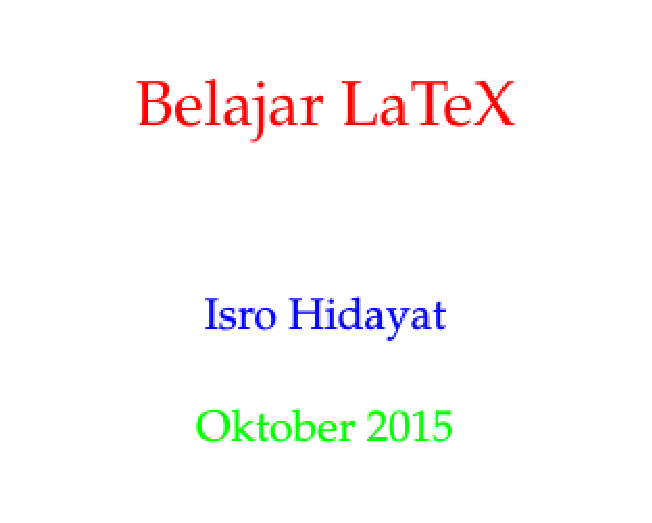
\includegraphics[scale=0.5]{package}
\caption{package.tex}
\label{fig:package}
\end{figure}

\section{Lingkungan \emph{Document}}
\subsection{Top matter}
Pada bagian paling awal dokumen ada informasi mengenai dokume itu sendiri, judul dan tanggal juga informasi mengenai penulis seperti nama, alamat dan email. Informasi ini lah yang dinamakan dengan \emph{top matter}

Contoh sederhana:
\begin{lstlisting}
\documentclass[11pt,a4paper]{report}

\begin{document}
\title{Belajar LaTeX}
\author{Isro' Hidayat}
\date{Oktober 2015}
\maketitle
\end{document}
\end{lstlisting}
Perintah \texttt{\textbackslash{}title} dan \texttt{\textbackslash{}author} biasanya diharuskan untuk diisi. Perintah \texttt{\textbackslash{}date} saja yang diketikkan, maka taanggal hari saat itu lah yang ditampilkan. Sedangkan perintah \texttt{\textbackslash{}maketitle} adalah penutup dari bagian top matter ini.

Ini adalah contoh yang lebih kompleks:
\begin{lstlisting}
\title{Cara Membuat Dokumen Menggunakan \LaTeX{}}
\author{Isro Hidayat\\
	Sekolah Rakyat\\
	Universitas Rakyat Kecil\\
	Buku\\
	Indonesia\\
	RN 98899\\
	\texttt{orsisam@gmail.com}}
\date{\today}
\maketitle
\end{lstlisting}
Tanda garis miring dua kali (\textbackslash{}\textbackslash{}) akan memaska LaTeX untuk ganti baris. Jika pengarang dokumen ada dua cara memisahkannya adalah dengan menggunakan perintah \texttt{\textbackslash{}and}:
\begin{lstlisting}
\title{Gawe Dewe}
\author{Cak Mat \and Cak Rupi'i}
\date{\today}
\maketitle
\end{lstlisting}

\subsection{Abstrak}
Pada kebanyakan lembar penelitian punya yang namanya abstrak. LaTeX telah menyediakan perintah untuk membuat abstrak, dan harus diletakkan pada susunan yang benar. Perintah ini diletakkan setelah top matter tapi sebelum bab utama. Perintah tersedia untuk class \emph{article} dan \emph{report} sedangkan buku tidak.
\begin{lstlisting}
\documentclass{article}

\begin{document}

\begin{abstract}
Di sini abtrak diletakkan...
...
\end{abstract}
...
\end{document}
\end{lstlisting}

LaTeX akan menggunakan kata \lq\lq Abstract\rq\rq\ sebagai judul secara default. Jika ingin merubahnya misal dengan nama \lq\lq Pengantar\rq\rq\ maka berikan perintah berikut sebelum memulai abstract.
\begin{lstlisting}
\renewcommand{\abstractname}{Pengantar}
\end{lstlisting}

\subsection{Pengaturan Bab}
Perintah \emph{sectioning} ini cukup beragam. Tergantung dari class dokumen masing-masing. Misal, class \texttt{book} punya perintah \texttt{\textbackslash{}chapter} sedangkan class \texttt{article} tidak. Berikut bentuk perintah sectioning ini:

\begin{lstlisting}
\chapter{Pengenalan}
Ini isi dari section chapter... 
Dalam bahasa indonesia ini lah yang dinamakan BAB

\section{SubBab}
Ini isi dari sub bab...

\subsection{SubsubBab}
Ini isi dari subsubbab...

\end{lstlisting}

Perlu diingat bahwa perintah sectioning ini tidak mengenal perintah pembuka(begin) atau penutup(end). Misal ketika kita mendeklarasikan perintah \texttt{\textbackslash{}chapter} maka secara otomatis menjadi Bab I sedangkan perintah \texttt{\textbackslash{}chapter} yang ke dua menjadi Bab II.

LaTeX menyediakan 7 level bab, seperti terlihat dalam tabel dibawah ini. Tiap bab pada tabek ini adalah subbab dari bab di atasnya.
\begin{table}[h!]
\caption{Susunan 7 Level Bab}
\centering
\begin{tabular}{l c l}
\hline\hline
\multicolumn{1}{c}{\bfseries Perintah} & \multicolumn{1}{c}{\bfseries Level} & \multicolumn{1}{c}{\bfseries Komentar}\\
\hline
\texttt{\textbackslash{}part\{\lq \lq part\rq \rq \}} & -1 & Tidak untuk class letter\\[1ex]
\texttt{\textbackslash{}chapter\{\lq \lq chapter\rq \rq \}} & 0 & Hanya book dan reports\\[1ex]
\texttt{\textbackslash{}section\{\lq \lq section\rq \rq \}} & 1 & Tidak untuk class letter\\[1ex]
\texttt{\textbackslash{}subsection\{\lq \lq subsection\rq \rq \}} & 2 & Tidak untuk class letter\\[1ex]
\texttt{\textbackslash{}subsubsection\{\lq \lq subsubsection\rq \rq \}} & 3 & Tidak untuk class letter\\[1ex]
\texttt{\textbackslash{}paragraph\{\lq \lq paragraph\rq \rq \}} & 4 & Tidak untuk class letter\\[1ex]
\texttt{\textbackslash{}subparagraph\{\lq \lq subparagraph\rq \rq \}} & 5 & Tidak untuk class letter\\[1ex]
\hline
\end{tabular}
\end{table}

Semua bab ini akan ditambahkan ke dalam daftar isi secara otomatis. Namun ini akan menjadi mesalah ketika kita membuat suatu perubahan standar, misal perubahan model pada heading, judul yang sangat panjang, ganti baris khusus atau font-font yang tidak normal. Perubahan ini akan juga terjadi pada daftar isi dan ini akan menyebabkan penataan pada daftar isi akan amburadul. Oleh karena itu LaTeX menyediakan sebuah judul alternatif, judul alternatif ini diletakkan pada kurung siku sebelum judul sebenarnya.
\begin{lstlisting}
\section[Judul Alternatif]{Judul Panjang Yang Sangat Panjang Sekali Sehingga Yang Membaca Jadi Capek}
\end{lstlisting}

\subsubsection{Penomoran Bab}
Penomoran bab pada LaTeX dilakukan secara otomatis, jadi jangan menambahkannya sendiri yah..!. Pada perintah \texttt{part} penomoran berupa huruf romawi (Part I, Part II, dst). \texttt{chapter} dan \texttt{section} berupa penomoran angka.

Kita bisa merubah seberapa penomoran bab yang ditampilkan, misal kita hanya ingin sampai 3 level penomoran (1.2.3.4.) maka perintah yang digunakan:
\begin{lstlisting}
\setcounter{secnumdepth}{3}
\end{lstlisting}
Mengapa sampai empat angka yang tercetak padahal cuma 3 level. Coba lihat tabel pe-level-an bab di atas, level ke 3 adalah subsubsection, jadi hanya sampai subsubsection ini sajalah penomoran yang terbentuk. Secara default penomoran ini hanya sampai level 2.

Ada juga yang namanya \texttt{tocdepth}, digunakan untuk menentukan sampai level berapa penomoran bab yang tercetak pada daftar isi. Cara mengubahnya pun sama yaitu:
\begin{lstlisting}
\setcounter{tocdepth}{3}
\end{lstlisting}
Sedangkan untuk mendapatkan bab yang tak bernomor dan tidak ditampilkan pada daftar isi. Tinggal ketikkan perintah diikuti tanda bintang * sebelum tanda kurung.
\begin{lstlisting}
\subsection*{Tidak Ikut Serta}
\end{lstlisting}
Semua versi perintah bab mulai dari \texttt{\textbackslash{}part*} sampai \texttt{\textbackslash{}subparagraph*} memiliki bentuk perintah ini.

Namun jika bab tak bernomor ini tetap ingin tercetak pada daftar isi, maka gunakan perintah \texttt{\textbackslash{}addcontentsline}:
\begin{lstlisting}
\section*{The Mask Man}
\addcontentsline{toc}{section}{The Mask Man}
\end{lstlisting}
\texttt{toc} bisa diganti dengan parameter lain misal \texttt{lot} untuk daftar tabel dan \texttt{lof} untuk daftar gambar.

Sebagai Catatan agar bookmark bisa bekerja dengan baik pada PDF agar bookmark dapat terhubung ke tempat yang tepat pada dokumen. Perintah \texttt{\textbackslash{}phantomsection} yang ada pada package \texttt{hyperref}, berikut implementasinya:
\begin{lstlisting}
\phantomsection
\addcontentsline{toc}{section}{Pengenalan}
\section*{Pengenalan}
\end{lstlisting}

Untuk perintah \texttt{chapter} kita harus memberikan perintah \texttt{\textbackslash{}cleardoublepage} untuk memperbaiki penomoran halaman pada daftar isi:
\begin{lstlisting}
\cleardoublepage
\phantomsection
\addcontentsline{toc}{chapter}{Dasar LaTeX}
\end{lstlisting}

Penomoran bab dapat diatur dimulai darimana dapat dilakukan dengan perintah:
\begin{lstlisting}
\setcounter{section}{4}
\end{lstlisting}
Bab selanjutnya setelah perintah ini akan diberi nomor 5.

\subsection{Paragraph Biasa}
Teks paragraf terletak setelah judul bab, hanya ketikkan beberapa kata atau kalimat. Untuk berganti paragraf hanya berikan baris kosong antar paragraf. Ini tidak akan berpengaruh pada berapa banyak jarak antar paragraf karena jarak diatur oleh format tersendiri.

\subsection{Daftar Isi}
Semua penomoran otomatis pada heading akan dimasukkan pada daftar isi secara otomatis. Untuk menambahkan daftar isi tinggal menambahkan perintah \texttt{\textbackslash{}tableofcontents}, bisanya setelah Abstrak atau Kesimpulan.

Perintah \texttt{\textbackslash{}listoffigures} dan \texttt{\textbackslash{}listoftables} punya fungsi yang sama pula dengan perintah \texttt{\textbackslash{}tableofcontents}, bedanya untuk menampilkan daftar gambar dan daftar tabel.

Untuk merubah judul daftar isi, karena pada dasarnya judul ini berbahasa inggris jadi agar berbahasa Indonesia kita harus merubah setting default judul daftar isi. cara merubahnya adalah dengan membubuhkan perintah \texttt{\textbackslash{}renewcommand\{\textbackslash{}contentsname\}\{Nama Judul Daftar Isi\}} pada bagian preamble. Sedangkan untuk daftar gambar, ubah \texttt{\textbackslash{}contentsname} dengan \texttt{\textbackslash{}listfigurename} dan daftar tabel dengan \texttt{\textbackslash{}listtablename}.

\subsubsection{Kedalaman Bab}
Kedalaman bab disini maksudnya adalah sampai level berapa kepala/judul bab yang tercetak pada daftar isi. Nah kedalaman bab pada daftar isi bisa diatur sampai seberapa yang tercetak, secara default sampai level 3. Cara merubah settingan default tersebut adalah dengan perintah:
\begin{lstlisting}
\setcounter{tocdepth}{4}
\end{lstlisting}
Perintah di atas menjadikan daftar isi mencetak header bab hingga pada level 4 yaitu paragraf. Sebagai catatan perubahan ini bersifat tetap, maksudnya berlaku untuk keseluruhan dokumen. Kita juga bisa merubahnya pada tipe bab tertentu saja:
\begin{lstlisting}
\makeatletter
\renewcommand*{\toclevel@chapter}{-1}	% membuat chapter se-level dengan part
\chapter{Hanya Chapeter Chappi}
\renewcommand*{\toclevel@chapter}{0}	% Mengembalikan level chapter ke semula
\makeatother
\end{lstlisting}

\section{Struktur Buku}
% 5.4 Structure Book - LaTeX.pdf halaman 60

\end{document}